\documentclass[conference]{IEEEtran}
% \IEEEoverridecommandlockouts
% The preceding line is only needed to identify funding in the first footnote. If that is unneeded, please comment it out.
%Template version as of 6/27/2024

\usepackage{cite}
\usepackage{amsmath,amssymb,amsfonts}
\usepackage{algorithmic}
\usepackage{graphicx}
\usepackage{textcomp}
\usepackage{xcolor}
% \usepackage{hyperref}
\usepackage[colorlinks=true, linkcolor=blue, citecolor=blue, urlcolor=blue]{hyperref}

\def\BibTeX{{\rm B\kern-.05em{\sc i\kern-.025em b}\kern-.08em
    T\kern-.1667em\lower.7ex\hbox{E}\kern-.125emX}}

\newcommand{\nsnote}[1] {{$\langle${\textcolor{blue}{NS: \textbf{#1}}}$\rangle$}}
\begin{document}

\title{Scalable Federated Fusion Planning for Decentralized Satellite-Based Ground Tracking\\
}

\author{\IEEEauthorblockN{ Nolan Stevenson}
\IEEEauthorblockA{\textit{ASEN 6519: Optimization: Applications and Algorithms} \\
\textit{University of Colorado Boulder} \\
}
}

\maketitle

\begin{enumerate}
    \item \href{https://github.com/nolans12/Satellite-DDF}{{\textcolor{blue}{Link to GitHub repository here.}}}
    \item \href{https://youtu.be/t9Bo5KCvhZA}{{\textcolor{blue}{Link to video here.}}}
\end{enumerate}

\section{Introduction}

% talk about satellite tracking and how it is a difficult problem to solve.

% Satellite-Based Ground Tracking is a cornerstone of modern Space Domain Awareness (SDA), enabling the detection, monitoring, and management of critical ground targets such as missile launches, military assets, and environmental threats. 
% By leveraging advanced space-based sensors, these systems provide a unique vantage point for tracking high-speed or concealed objects, offering real-time intelligence that is essential for national security, disaster response, and strategic operations. 
% However, this field is filled with challenges, including the need to accurately fuse measurements from multiple satellites, respond to dynamic threats online, and manage the limitations of satellite compute and communications.
% Additionally, all of these problems typically need to be acomplished autonomously; to expedite speed and response. 
% This paper will be discussing how compute and communication limitations can be addressed by leveraging optimization and data fusion techniques.


Satellite-Based Ground Tracking is a cornerstone of modern Space Domain Awareness (SDA), enabling the detection, monitoring, and management of critical ground targets such as missile launches, military assets, and environmental threats. 
By leveraging advanced space-based sensors, satellites can collect high vantage point measurements on potential targets. These measurements are then processed by advanced data fusion algorithms that are able to generate a high-fidelity track of an object.
This allows real-time intelligence that is essential for national security, disaster response, and strategic operations.
However, this field is filled with challenges, including the need to accurately fuse measurements from multiple satellites, respond to dynamic threats online, and manage the limitations of satellite compute and communications.
Additionally, all of these problems typically need to be acomplished autonomously; to expedite speed and response. 
This paper will be discussing how compute and communication limitations can be addressed by leveraging optimization and data fusion techniques.



\section{Background and Related Work}

\subsection{Centralized Data Fusion}

% Talk about standard centralized fusion approaches.
% Algorithms such as EKF, etc. networking setup.

The most common approach for SDA tracking applications is a centralized approach. 
In this approach, measurements from a common region or satellite are sent to a ground station where a powerful computer is able to run state of the art data fusion algorithms.
This allows the highest quality filters to be ran on the data, allowing for super high fidelity tracking. 
Additionally, the algorthimic approach is quite simple and easy to implement, imagine just a single Extended Kalman Filter (EKF) \cite{b5} running a batch update on hundreds of measurements all at the same time.
This approach also allows easy communication protocols for satellites on where they should send their measurements too; you just always send it to the centralized ground station.

The centralized architecture was primarily designed around a human operator. With a centralized location for all data management and fusion, an operator can easily monitor the system and make decisions.
Some decisions an operator might make would be which friendly assets should recieve certain data about an enemy target, where should the sensors on the satellites be pointed, and which areas of the globe should be given a higher priority.

However, there are several negative aspects to this approach. First, the system has a critical point of failure. All measurements and tracks exist and are processed at a single point,
which means if that point is compromise the whole system fails. Additionally, the system has a large amount of inertia in decision making and processing. Waiting for a human operator to make a decision can cost time which is extremely valuable in a warfighting environment.
Also, when critical information needs to be sent to friendly assets, that data first has to be sent from satellite to ground station for processing, then from ground station back to a communication satellite that can relay the information to the reqeusting asset.

\subsection{Decentralized Data Fusion}

An alternative approach to centralized data fusion is decentralized data fusion (DDF). In DDF, individual agents run their own estimation algorithms on the data they collect or recieve.
Then, collabratively, these agents communicate with each other to reconsile their information into a better single estimate. DDF is widely used in multi-agent systems where agents are able to sense, communicate, and process information \cite{b1}.

\begin{figure}[h]
    \centering
    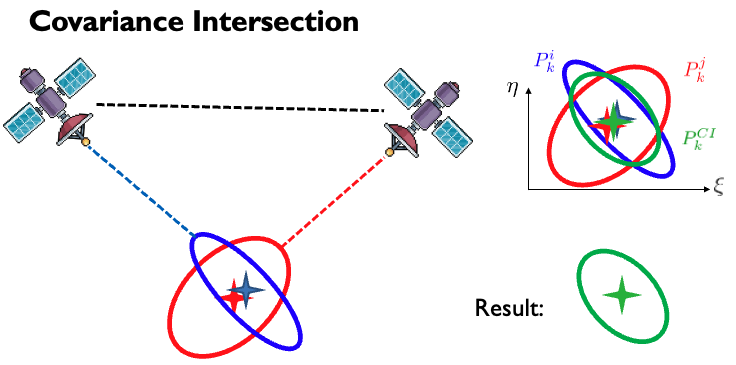
\includegraphics[width=0.35\textwidth]{figs/covariance_intersection.png}
    \caption{Covariance Intersection Fusion to combine two mono tracks into a fused track. The blue and red ellipses are the covariance of the two estimates. The green ellipse is the resulting covariance of the fused estimate. }
    \label{fig:ci_fusion}
\end{figure}

In the context of SDA applications, DDF may be useful for tracking ground targets. If each satellite was intelligent enough to run its own onboard estimation algorithm, such as an EKF,
then the satellites could communicate with each other to reconsile their information into a better single estimate.
This is particularly useful for satellites as measurements taken by satellite sensors are typically bearings only measurements. 
A bearings only measurement is just a line of sight vector from a satellite to a location in the sensor frame.
By itself, a bearings only measurement is not enough to estimate a 3D position as there is a missing dimension, but, when combined with multiple measurements, especially from different viewing angles, the 3D position can be reconstructed.
In the satellite tracking context this is known as upgrading a track from a mono-track to a stereo-track, giving it multiple dimensions of information.
The DDF algorithm covariance intersection (CI), shown in Figure~\ref{fig:ci_fusion}, is a widely used algorithm that employs this strategy and has been the state of the art for DDF applications for over 25 years \cite{b4}. 

If the DDF approach was implemented in a satellite network, it would allow for much more robust tracking and agile decision making. By decentralizing the data and information, you remove the critical point of failure in the system. 
Also, if the critical information is processed in the sky user requests for data can be quickly transmitted, instead of having to go back and forth with a ground station system.


% Talk about decentralized fusion approaches.
% Algorithms such as covariance intersection and et-ddf.
% How these approaches are used in the cooperative tracking domain.



\section{Problem Formulation}

With new innovations in satellite technology, from higher processing power to tactical data links capable of communicating with ground assets \cite{b10} to rapid deployment via reusable rockets, the potential for proliferated satellite networks 
capable of performing decentralized data fusion is becoming more realistic.
The case we will consider in this paper is a global coverage LEO satellite network with high processing power and communication capabilities. 
The goal of this network is to track ground targets of interest, doing all fusion, sensing, communication, and planning in the sky.

\subsection{The Fusion - Sensing Layer}

% talk about how this layer can help seperate or solve the typical DDF problem.

% How in this layer, talk about compute vs sensing etc. 

    % \begin{figure}[h]
    %     \centering
    %     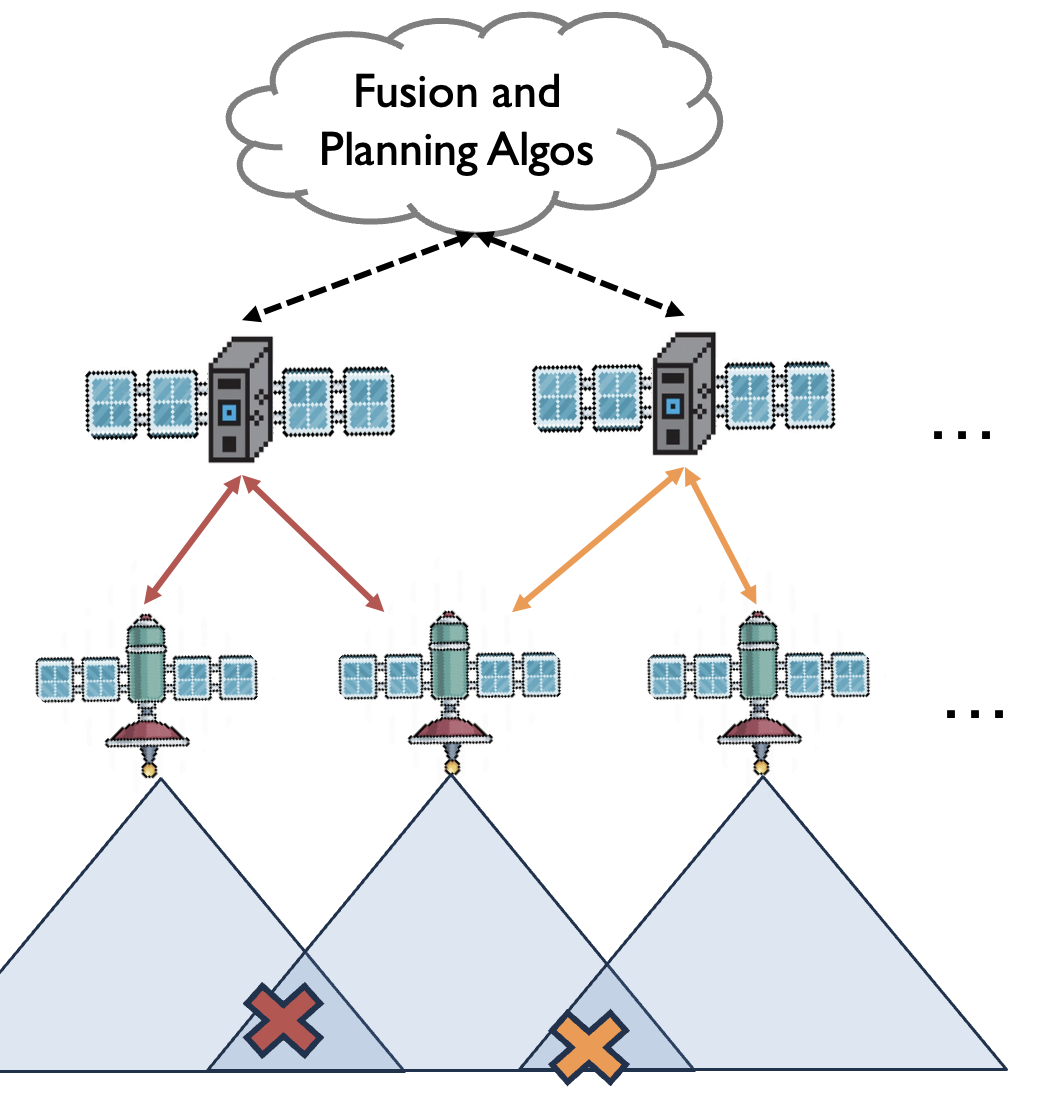
\includegraphics[width=0.35\textwidth]{figs/fusion_sensing_arch.png}
    %     \caption{Fusion - Sensing Architecture. The sensing layer is able to take measurements on targets (Xs) and communicate that back to the fusion layer. }
    %     \label{fig:satellite_structure}
    % \end{figure}

    The satellite network can be broken up into two layers of satellites; a sensing layer and a fusion layer. 
    The sensing layer consists of satellites that have powerful sensors capable of taking measurements on ground targets. 
    The fusion layer consists of satellites that have higher computational and communication capabilities allowing them to fuse measurements from the sensing layer. 

    The role of the sensing layer is to take measurements on ground targets. The sensing layer may contain a variety of sensors, 
    but, for simplification, we will assume all measurements taken are a bearings only measurement; a line of sight vector from a satellite to a predicted ground target.
    Once a sensing satellite has a measurement, it needs to communicate this measurement to the fusion layer for processing. 
    The fusion layer has the capability to recieve multiple measurements and generate an accurate track estimate using an Extended Kalman Filter. 
    The fusion nodes are also responsible for maintaining consistency in the track estimates. 
    This means that if two fusion nodes have conflicting track estimates, they must be reconciled using data fusion techniques such as covariance intersection, as mentioned in the background section.

\subsection{Federated Fusion}

% talk about how strcutred in a federated fusion approach. 

    \begin{figure}[h]
        \centering
        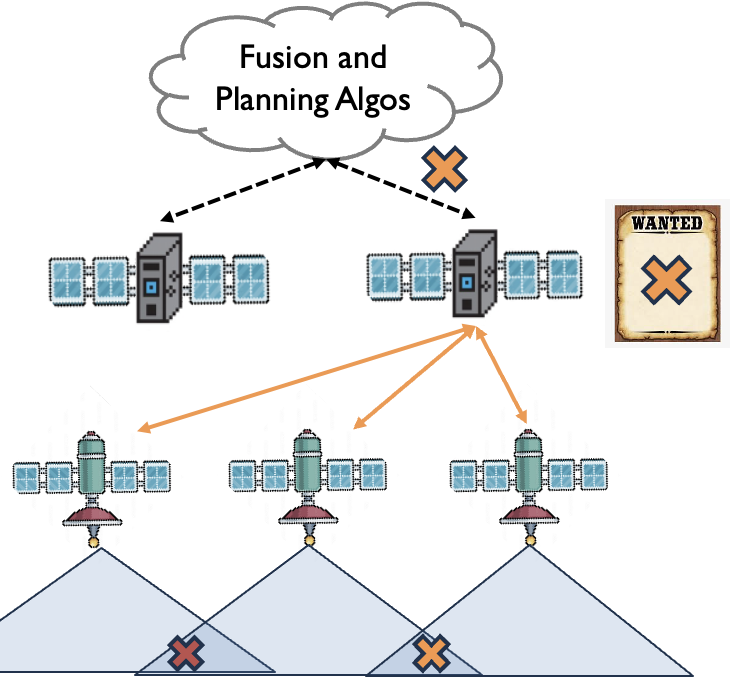
\includegraphics[width=0.35\textwidth]{figs/custody_bounty_sys.png}
        \caption{Federated Fusion Architecture. The fusion layer plans for custody, and assigns custody of the orange target to the right fusion node. This custody is then communicated to the sensing satellites. So that when those sensing satellites take a measurement on the orange target they send that to the fusion node that has custody of that target. }
        \label{fig:custody_bounty_sys}
    \end{figure}


    Federated fusion is a method of decentralized data fusion that allows for a dynamic programming type approach to data fusion.
    Instead of one centralized node being in charge of all tracks, sub-clusters of nodes can be assigned tasks.
    In the satellite tracking problem, federated fusion can be used to assign specific fusion nodes to be responsible for a specific track or region.
    If a fusion node is assigned a track, it will be the primary reciever of all measurements associated and will be responsible for the data fusion algorithms mentioned in the background section.
    Once a fusion node has been assigned "custody" of a track, all neccessary sensing satellites must be alerted of this. 
    Thus, when the sensing satellites take a measurement on that target or region, they know who to relay that data to in the fusion layer. 
    This entire process, which is called the "Custody-Bounty" system, is shown in Figure~\ref{fig:custody_bounty_sys} where the fusion nodes are shown with computers, the sensing satellites are shown with camera FOVs, and the targets are shown with Xs. 

    The key algorithm that is needed for this system to work is the ability to intelligently assign custody of targets to fusion nodes.
    Custody must be assigned while considering the computation constraints of the fusion nodes, each fusion node can only track a small number of targets due to computation limits.
    Additionally, communication limitations must also be considered. Satellites in a LEO constellation are able to communicate with eachother through a nearest neighbor communication network.
    Thus, if data needs to be sent a long distance in the network, it has to travel through multiple hops, which increases latency and bandwidth.
    
    The problem that will be addressed in this paper is how to assign custody of targets to fusion nodes while considering the computation and communication limitations of the system.
    
    % The communication links for a LEO satellite are limited, generally just neighbor to neighbor communication.
    % If communication has to travel further in the network, through multiple hops, latency will increase in the transmission, which impacts the performance of the fusion algorithms.
    % Thus, the problem that wille be addressed is how to assign custody of targets to fusion nodes while considering the computation and communication limitations of the system.


\subsection{Simulation Environment}

    To test the impact of federated fusion and optimization techniques, a Python simulation environment was created. 
    The class structure of this simulation environment is shown in Figure~\ref{fig:simulation_environment}.

    \begin{figure}[h]
        \centering
        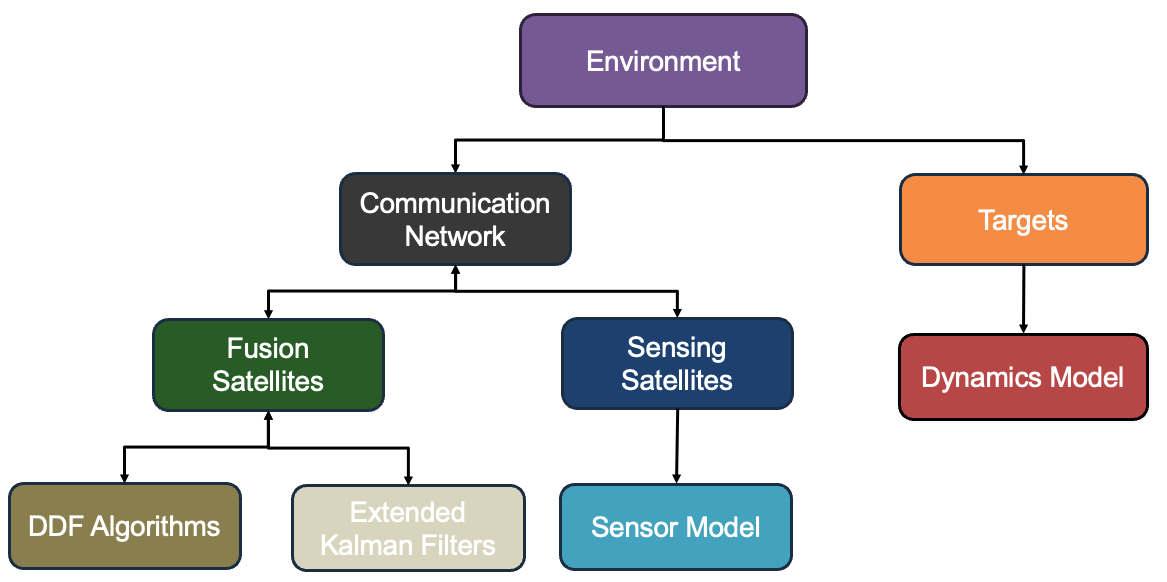
\includegraphics[width=0.45\textwidth]{figs/code_class_heirarchy.png}
        \caption{Simulation Environment Class Heirarchy}
        \label{fig:simulation_environment}
    \end{figure}

    This simulation environment is able to simulate scenarios with a large number of satellites and targets.
    All targets are given random spherical dynamics with speeds ranging from 0.3 to 5 Mach.
    Sensing satellites with sensors are able to take noisy measurements on these targets given by their sensor FOV and bearings errors.
    These measurements are then able to be sent through a realistic nearest neighbor communication network to fusion nodes.
    The fusion nodes are capable of taking batches of measurements and running extended kalman filters to generate track estimates. 
    Fusion nodes can also combine estimates from neighboring nodes using distrbuted data fusion (DDF) algorithms such as covariance intersection to generated a consistent track estimate.
    Assuming the fusion nodes are able to communicate in a centralized manner for planning, an algorithm can be used to assign custody of each estimated target to fusion nodes.
    Once custody is assigned, sensing satellites are given this information as a protocol of who to send their measurements to; allowing the federated fusion system to work.
    Thus, this simulation environment is capable of simulating a large variety of scenarios neccessary for the purpose of this paper, all future results and plots will be generated from this simulation environment.

    All code for this simulation environment is available via the GitHub link at the top of the paper.
    


\section{Solution Approach}

\subsection{Mixed-Integer Linear Program To Minimize Comms}

    % the full formulation of the milp

    The satellite-target custody problem can be solved used a mixed-integer linear program (MILP). 
    The performance parameters the system is trying to optimize is to minimize the communication costs of the system while also staying under computational limitations.
    In general, this type of satellite constellation is more limited by computation than communication, as there are many options for routing comms throughout neighboring nodes, but much harder constraints on the computational capacity of a satellite.
    Thus, the algorithm presented will set a hard constraint on the number of targets a fusion node can track, and then optimize to minimize communication costs to account for both the communication and computational performance.

    The MILP can be formulated as follows:

    \begin{equation}
        \underset{x_{st}}{\text{minimize}} \sum_{s} \sum_{t} c_{st} x_{st}
        \label{eq:objective}
    \end{equation}
    
    \text{subject to}

    \begin{equation}
        x_{st} \in \{0, 1\} 
        \label{eq:binary}
    \end{equation}

    \begin{equation}
        \sum_{s} x_{st} \geq 1 \quad \forall t
        \label{eq:constraint1}
    \end{equation}

    \begin{equation}
        \sum_{t} x_{st} \leq Comp(s) \quad \forall s
        \label{eq:constraint2}
    \end{equation}

    In the formulation above, $s$ is the index for a fusion satellite, and $t$ is the index for a target. \\
    Equation~\eqref{eq:objective} is the objective function, which is to minimize the cost of assigning custodies throughout the network (more dicussion on that cost below). \\
    Equation~\eqref{eq:binary} is the binary constraint, which ensures that the decision variable $x_{st}$ is either 0 or 1. If $x_{st} = 1$, then fusion satellite $s$ has custody of target $t$. \\
    Equation~\eqref{eq:constraint1} ensures that every target has at least one fusion satellite assigned to it. This means that each target is being tracked in the network. \\
    Equation~\eqref{eq:constraint2} ensures that no fusion satellite is assigned more targets than its computational limit, defined as $Comp(s)$. 

    The cost of assigning custody of a target to a fusion satellite is defined as $c_{st}$. A good cost function is one that minimizes the amount of communication throughout the network. 
    Since the goal of the algorithm is to assign custodies for some short horizon into the future, the cost function needs to account for current and future communication needs. 
    A simple choice for the cost function over some planning horizon $T$ is:
    \begin{equation}
        c_{st} = \sum_{k=0}^{T} \| \mathbf{r}_k^{target} - \mathbf{r}_k^s \|
        \label{eq:cost}
    \end{equation}

    The cost function is the sum of the distance between the estimated target position and the fusion satellite position over a discrete set of points from current time into the future horizon. 
    Future target position can be estimated by using the output of the track fusion algorithms. A extended kalman filter, as used in this paper, is able to output the estimated spherical dynamics of the targets, so this can be propagated forward in time to get an estimate of target position.
    Future satellite position is more easily known due to theconstant orbital parameters of a given satellite.
    This cost function is a good proxy for communication cost because it is a approximation for how far the measurement data needs to travel until it reaches the destination fusion satellite, thus, acting as a proxy for communication hops in the network. 
    By minimizing communication travel distance and number of hops, we are effectively minimizing the bandwidth usage and latency of the system.

\subsection{Overcapacity Case: Including Target Priority}

    % the full formulation of the milp with regional priority and how regional priority is included
    % also the modification 

     Although the above MILP is a good start, it does not account for scenarios where the number of targets requested to track is greater than the capacity of the system. 
     This is a very important edge case to consider and one that is often likely to happen in a real-world raid scenario.
     In a overcapacity case, the choice has to be made on which targets to track and which to not track. 
     Thus, the best way to solve this problem is to include notions of importance on the targets.

     To assign priority for targets, we will assume a priority is given to areas across the globe. Therefore, if a target is within that region, it is given the priority associated with that region.
     To implement priorities into the optimization problem, we will add a scaling factor, $f_{t}$, into the cost function which can account for this priority.
    
     \begin{equation}
        \underset{x_{st}}{\text{minimize}} \sum_{s} \sum_{t} c_{st} x_{st} \textcolor{red}{f_{t}}
        \label{eq:objective_priority}
    \end{equation}
    The priority factor function, $f_{t}$, can be defined as the following equation for a given target priority $p_{t}$:
    \begin{equation}
        f_{t} = X^{p_{t} - 1}
        \label{eq:exchange_rate}
    \end{equation}

    Equation~\eqref{eq:exchange_rate} is a good proxy to account for the impact of priorities on the cost function.
    The term $X$ is called the "exchange rate" and it's a constant that gives the relative importance of a priority level and the next priority level.
    I call it the exchange rate because it is the factor that scales the costs between priority levels.
    For example, if $X = 2$, then a target with priority 3 has 2 times the cost of a target with priority 2.
    Thus, a external user to the system can scale this exchange rate to give more or less weight to priorities, as desired.
    A graph showing the cost of varying priorities depending on the exchange rate is shown in Figure~\ref{fig:priority_cost}.
    
    \begin{figure}[h]
        \centering
        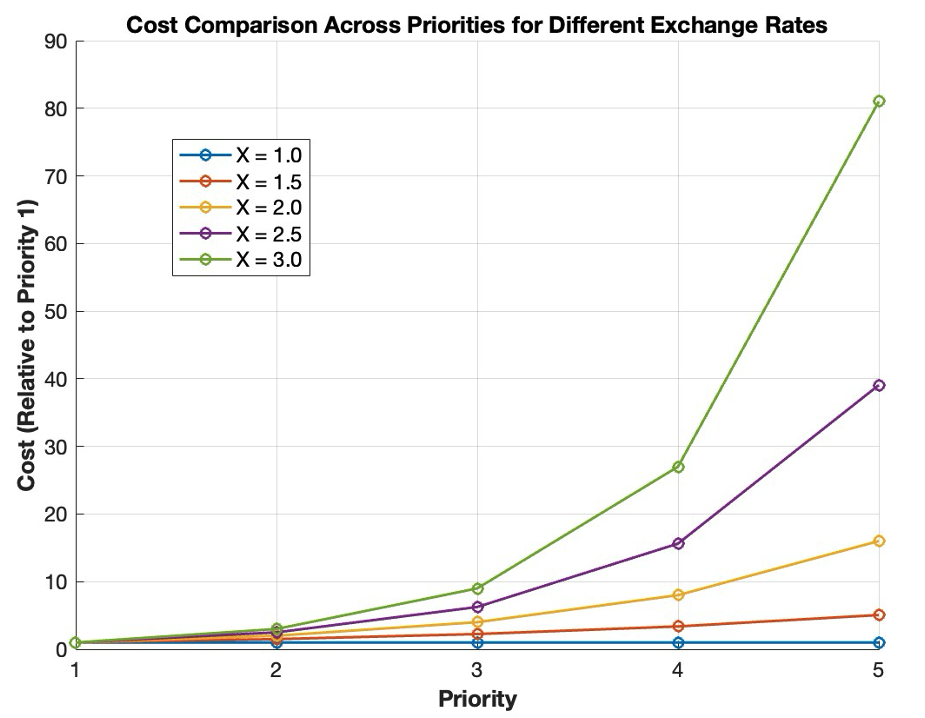
\includegraphics[width=0.5\textwidth]{figs/cost_vs_priority.png}
        \caption{Impact on exchange rate on the relative cost of priority levels}
        \label{fig:priority_cost}
    \end{figure}

    Additionally, the MILP needs to be modified to account for the overcapacity case.
    No longer, is the constraint given in Equation~\eqref{eq:constraint1} valid, as not every target can be tracked.
    Instead, the new constraint is given by:
    \begin{equation}
        \sum_{s} \sum_{t} x_{st} == \sum_{s} Capacity(s)
        \label{eq:constraint_overcapacity}
    \end{equation}

    Where $Capacity(s)$ is the computational capacity of the fusion satellite $s$. This new constraint ensures that the system is able to track as many targets as possible, fully saturating the satellites.

\subsection{Optimization Solver}

    %  talk about how used PuLP to solve the MILP, how pulp used branch and bound to solve the MILP

    The two MILP formulations presented above can be solved using off the shelf solvers. 
    Since the problem setup is in Python, as mentioned in the Problem Formulation section, a Python package called PuLP is used to solve the MILP \cite{b6}.
    PuLP is a Python package that is used to solve linear programming problems.
    This package uses the COIN-OR Branch and Cut Solver, which is a state-of-the-art solver for mixed-integer linear programs.
    This package uses open source mathmatical tools given by the Computational Infrastructure for Operations Research (COIN-OR) project \cite{b2}.  
    With these tools, the Branch and Cut algorithm is able to solve the MILP to global optimality, meaning that the solution is the optimal solution to the MILP.
    An example of how the Branch and Cut algorithm works is shown in Figure~\ref{fig:branch_and_cut}. 
    The algorithm works by first solving a linear program without the integer constraints using the Simplex algorithm \cite{b7}.
    Then, when a solution to the relaxed problem is obtained, a cutting plane algorithm is able to splice the solution by integer planes.
    This process is repeated until a solution is found that satisfies all constraints.

    \begin{figure}[h]
        \centering
        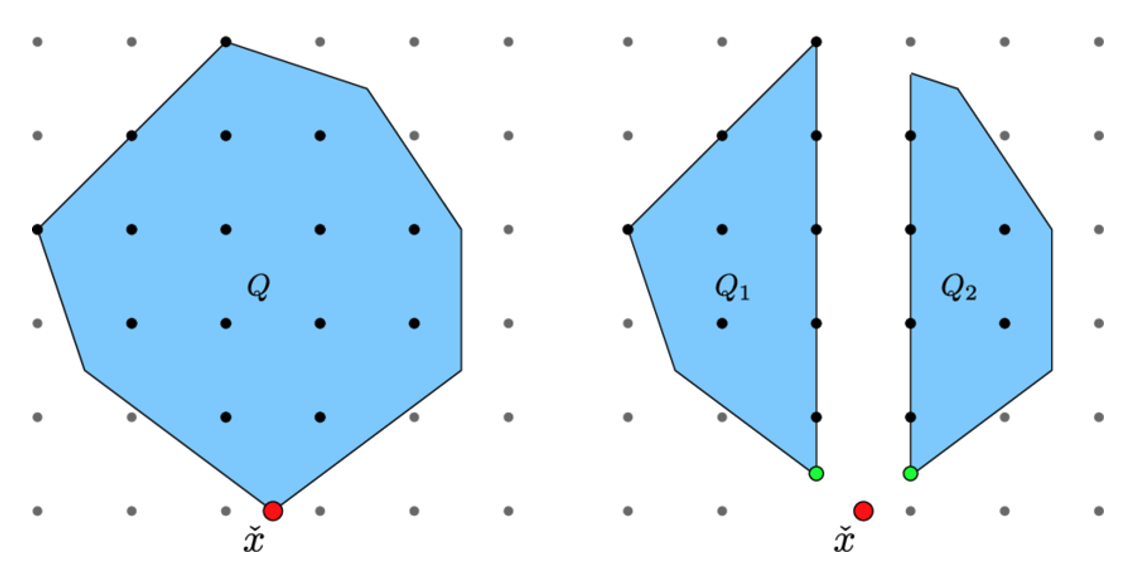
\includegraphics[width=0.45\textwidth]{figs/branch_and_cut.png}
        \caption{Branch and Cut Algorithm: cutting planes to get integer constraints}
        \label{fig:branch_and_cut}
    \end{figure}

\section{Results}

    All results were generated by simulating a 200 satellite enviornment; 100 sensing satellites and 100 fusion nodes.
    The sensing satellites follow a 45 degree inclination, 1000 km altitude walker-delta constellation composed of 5 planes each with 20 satellites.
    Each sensing satellite has a bearings only sensor on it with a diagonal FOV of 115 degrees. Bearings measurements are taken as truth data of the target with added white noise of +- 0.115 degrees in either bearings angle direction (in-track angle and cross-track angle).
    The fusion satellites follow a 90 degree inclination, 1000 km altititude walker-delta constellation composed of 5 planes each with 20 satellites.
    Each fusion node has a maximum computational capacity of 2 tracks; meaning it can only handle 2 extended kalman filters at a time. 
    The communication network is a nearest neighbor network, with a maximum communication range of 1000 km and a maximum number of neighbors of 4.
    The scenario simulated has 5 countries spawning targets with random spherical dynamics: the United States, China, Ukraine, South Africa, and Argentina.

    The custody assignment MILP was reran every 1 minute in the simulation based on all avaliable target tracks throughout the fusion network.
    The planning horizon used for each MILP solution was also 1 minute.
    In scenarios where multiple fusion nodes have differenting target tracks, covariance intersection was used to reconcile the tracks, allowing planning under consistent knowledge.

\subsection{Undercapacity Case}

    % here show the results for how the milp performs in the undercapacity case. 

    % also show the scalability of the solver. 
    % a plot for time to solve solution and also a plot showing how the federated system performs.

    To test the performance of the MILP algorithm for a nominal, undercapacity case, each country was given 20 targets. 
    Every 1 minute in the simulation, a new custody plan was generated using the MILP algorithm. 
    The initial custody plan that was generated is shown in Figure~\ref{fig:initial_custody_nominal}.

    The targets are colored according to their country of origin, as shown in the legend.
    All sensing satellites are shown in a very dim blue, all fusion satellites without custody are shown in a very dim green. 
    The fusion satellites that were assigned custody of targets are colored the same as the targets they are assigned to.
    The black lines indicate communications of measurements on targets from the sensing layer to fusion nodes with custody.

    These results look to be succcessful, as all targets are being tracked by at least one fusion node. 
    Additionally, the fusion nodes that were assigned custody are close to the targets they were assigned, as optimized in the cost function. 
    This is able to reduce the amount of communication hops required for a measurement to reach the fusion node.
    
    We can also compare our solution from the MILP in a federated fusion architecture to that of a typical decentralized data fusion (DDF) architecture.
    Where in this typical DDF architecture, no custodies are assigned, instead, all fusion nodes run EKFs on every measurement they recieve. The sensing nodes send measurements they takes to the nearest fusion node in communication range.
    Thus, there is issues of track consistency in the network as you may have multiple fusion nodes tracking the same target using different measurements.
    This means that at each time step, the fusion nodes reconsile their independent tracks together using pairwise covariance intersection. 
    This pairwise covariance intersection was simulated alongside the federated MILP solution to see how the two architectures perform in the exact same scenarios.
    The results comparing the average fusion time of the per fusion node per time step are shown in Figure~\ref{fig:federated_vs_ddf}.

    \begin{figure}[h]
        \centering
        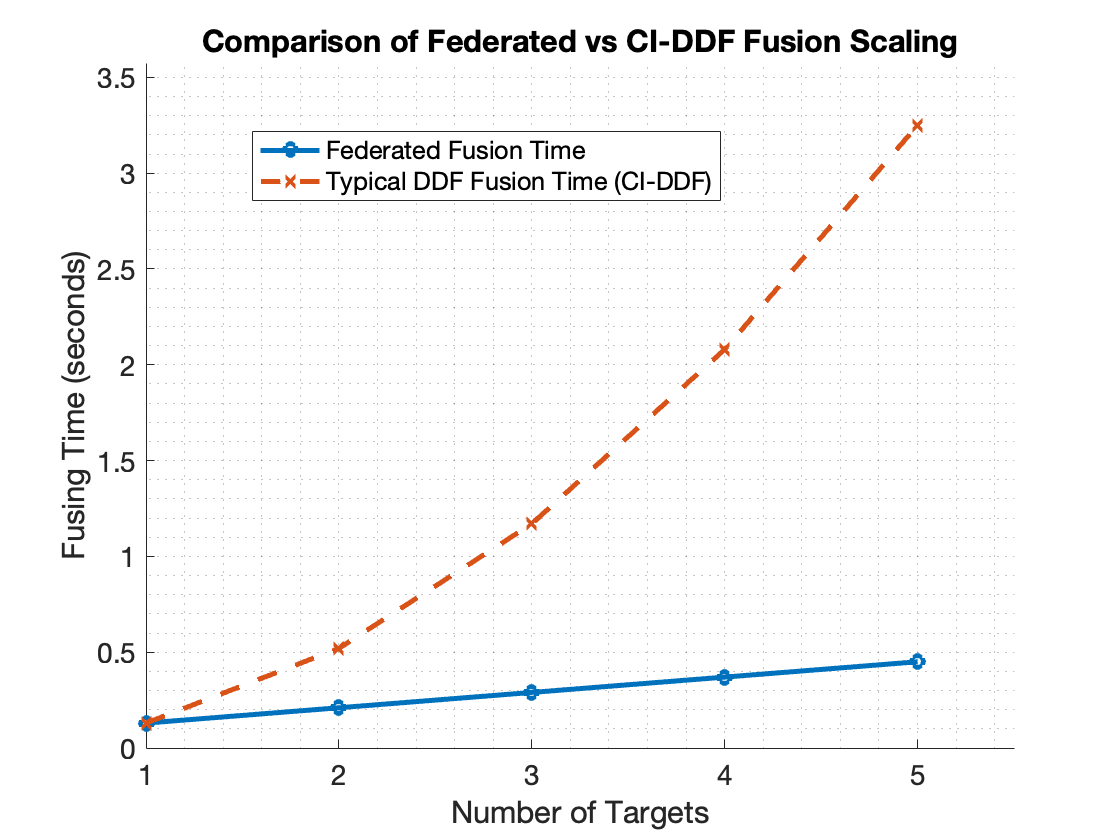
\includegraphics[width=0.5\textwidth]{figs/ci_vs_federated.png}
        \caption{Average fusion time per fusion node per time step for the federated MILP solution vs the CI DDF solution.}
        \label{fig:federated_vs_ddf}
    \end{figure}

    The results show a massive improvement to scalability when using the federated architecture with the MILP algorithm to assign custody. 
    The behavior of the DDF solution is about $O(N^2)$ with $N$ number of targets. This makes sense as each fusion node has to combine its tracks with neighboring fusion nodes each time step, leading to more communication and computation.
    The federated solution on the other hand is about $O(N)$ with $N$ number of targets. The custody-bounty system allows an average of 1 data fusion algorithm, such as an EKF, to be run per target, and little pairwsie fusion is required.

\subsection{Overcapacity Case}

    % show the plot of priority assignments vs exchange rate.
    % maybe show a plot showing how the system looks with a higher exchange rate?

    To test the performance of the MILP algorithm for an overcapacity case, each country was given 100 targets. 
    Additionally each country was assigned a priority, with the United States having a priority of 1, China having a priority of 2, Ukraine having a priority of 3, South Africa having a priority of 4, and Argentina having a priority of 5.

    For this overcapacity case, which targets the system chooses not to track is influenced heavily on the exchange rate, as formulated in Equation~\eqref{eq:exchange_rate}.
    Plots showing the custody assignments of the network for an exchange rate of 1 vs an exchange rate of 1.6 are shown in Figures~\ref{fig:exchange_rate_1} and \ref{fig:exchange_rate_1.6}.
    The relationship between the exchange rate and the number of targets tracked in each of the countries is shown in Figure~\ref{fig:assignment_vs_exchange_rate}.

    \begin{figure}[h]
        \centering
        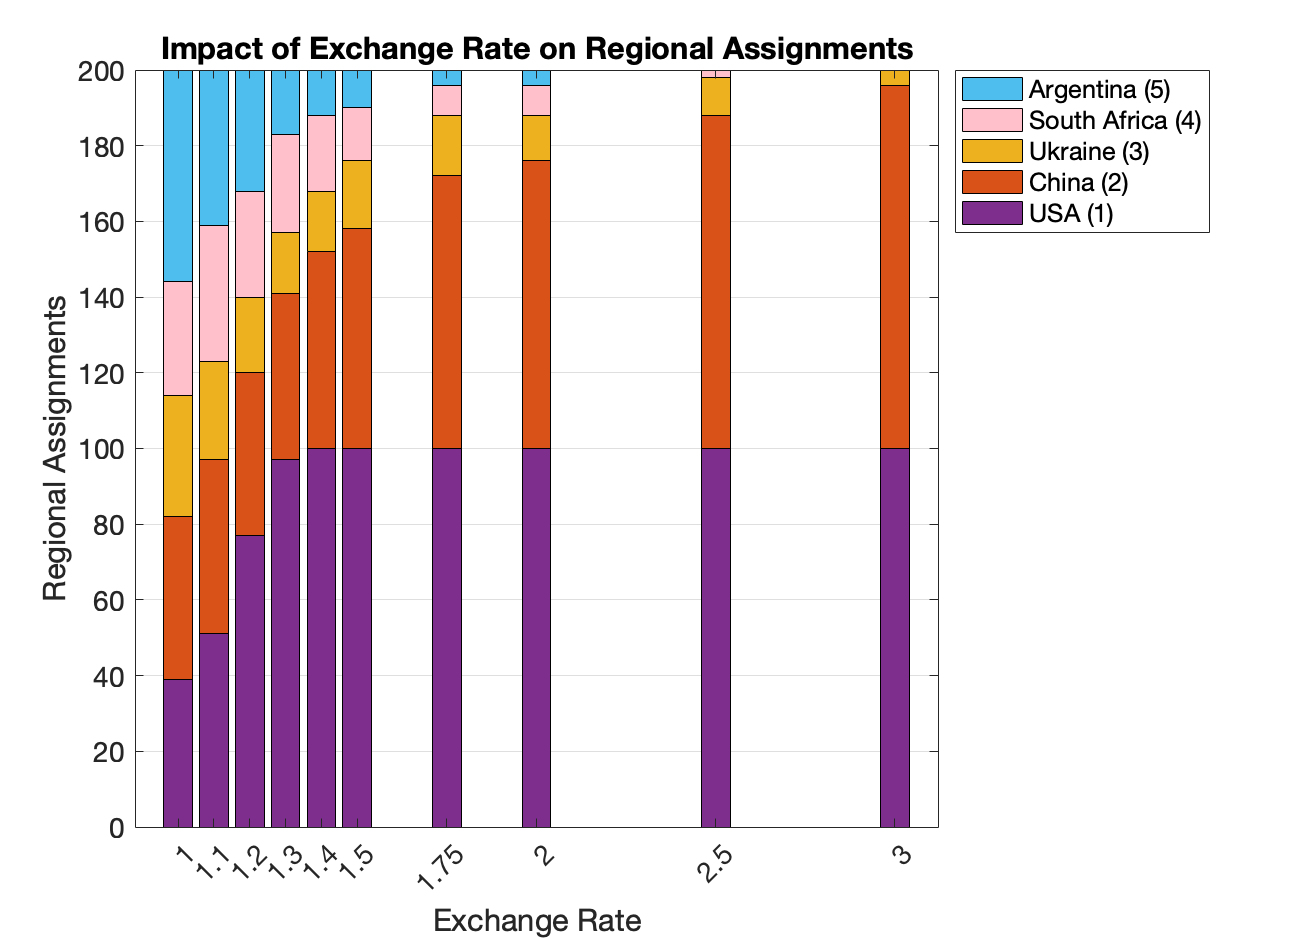
\includegraphics[width=0.5\textwidth]{figs/assignment_vs_exchange_rate.png}
        \caption{Relationship between number of targets tracked per country vs the exchange rate. Countries were given the priorities listed in the legend.}
        \label{fig:assignment_vs_exchange_rate}
    \end{figure}

    The results show that as the exchange rate increases in the system, the strength of the priorities in assigning targets increases. 
    This is a successful result as it shows the system is able to be adjusted to the needs of the user. 
    Depending on the exchange rate set by a user, the system can be adjusted to ensure the degredation in tracking targets matches the user's needs.

    However, it is important to note that by increasing the exchange rate and giving more weight to priorities, the system produces a worst result for minimizing communications. 
    The original MILP formulation wihtout priorities is design specifically to minimize communicaitons by using the proxy cost function given in Equation~\eqref{eq:cost}.
    By scaling this cost function with the priority factor, the solution is no longer optimal with resepct to that proxy function. 
    The relationship for the average communication distance travelled by a measurement through the network from sensing node to custody node is shown in Figure~\ref{fig:comm_distance_vs_exchange_rate}.

    \begin{figure}[h]
        \centering
        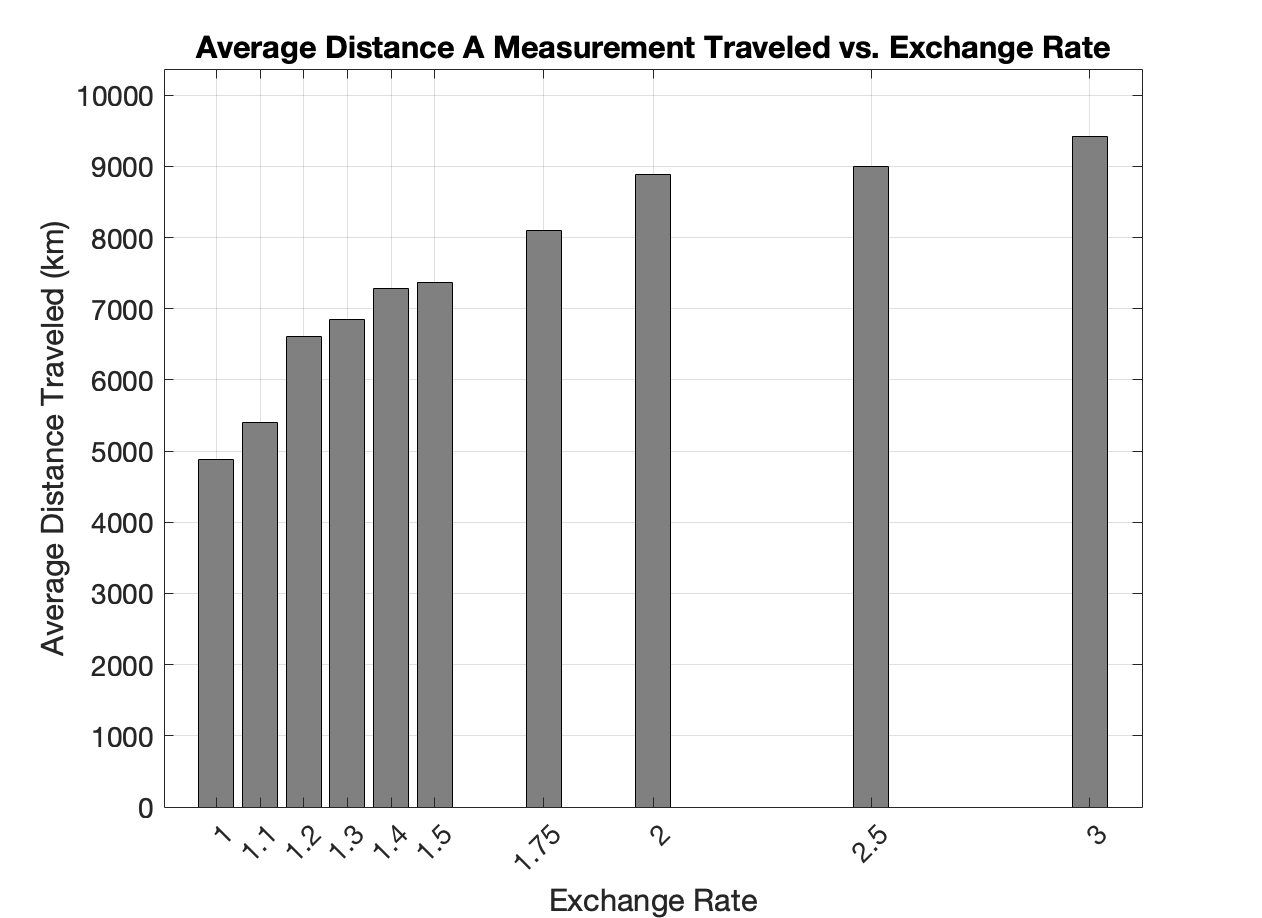
\includegraphics[width=0.5\textwidth]{figs/distance_vs_exchange.png}
        \caption{Average communication distance traveled by a measurement through the network from sensing node to custody node for a variety of exchange rates.}
        \label{fig:comm_distance_vs_exchange_rate}
    \end{figure}

    The results show for this overcapacity case, as the exchange rate increases, the average communication distance traveled by a measurement increases. 
    This result can be better visualized by looking at the custody plan for the exchange rates of 1 and 1.6, shown in Figures~\ref{fig:exchange_rate_1} and~\ref{fig:exchange_rate_1.6}.
    In these plots, you can see that at a higher exchange rate, the nodes assigned custody of the USA and China begin taking over the regions previously assigned to Argentina and South Africa. 
    While this happens due to the priority scaling, this decreases communication efficiency, thus, increasing latency and bandwidth usage. However, a higher number of higher priority targets are being tracked; 
    this is the resulting trade off that occurs when increasing the exchange rate. 

    A video showing the results of scaling the exchange rate online in the simulation environment is available at the top of the paper.

\section{Conclusion and Future Work}
\subsection{Conclusion}

% talk about how this solves the problem of scalability when coupled with the federated system.
In conclusion, this paper showed a method to plan for fusion in a decentralized satellite-based ground tracking system. 
With continual improvements to satellite technology, decentralized satellite networks are the future of space domain awareness and tracking, thus, it's important to establish algorithms that can manage these massive proliferated networks.
This paper showed a optimization approach to plan for data fusion across a distrbuted network of compute nodes.
The algorithm was able to obey computational constraints per fusion node while also minimizing communication costs throughout the network.
Additionally, the federated fusion structure presented in this paper when combined with this algorithm was able to solve the problem of scalability that so many other decentralized data fusion systems face, as seen in Figure~\ref{fig:federated_vs_ddf}.

The basic fusion planning algorithm was also extended to account for different target priorities, which allows for the system to be adjusted to the needs of the user.
It was shown that by incorporating a scaling factor into the algorithm to account for target priorities, given in Equation~\eqref{eq:exchange_rate}, the system was able to degrade in tracking targets in the correct manner if given an oversatured environment, as shown in Figure~\ref{fig:assignment_vs_exchange_rate}.
Thus, a external user to the system could tune the exchange rate to match thier needs, whether that be minimizing communication costs or prioritizing tracking important targets.

The algorithm presented in this paper relies on the specific fomrulation of the satellite network that was presented in the Problem Formulation section.
This paper thus also showed a way to formulate a satellite network with the federated fusion architecture, which allows for advanced task assignment algorithms to be used.

\subsection{Future Work}

Although the algorithm and results presented in this paper are a successful start to planning for distrbuted fusion in a satellite network, there are many areas for future work.

\subsubsection{Further Work on Target Priorities}
The scenarios presented in this paper used the simplification that regions of the globe have a given prioritiy and targets existing in that region are assigned the same priority.
However, there are more advanced ways to assign priorities to targets.
In defense applications, priority of targets is not a function of where a current target is, but, where it is going; especially in missile defense applications.
A scenario could be fomrulated where there are regions of defense priority. 
Then, based on the estimated target dynamics, from fusion algorithms, the priority of a target is a function of which defense region the target appears to be headed towards.
This would be a more advanced way to assign priorities to targets. 
Once priorities are assigned to targets, the algorithm presented in this paper would be able to optimize accordingly.


\subsubsection{Account for Raid Uncertainty}
The solution presented in this paper assumes a constant, known, amount of targets are planned for over some given horizon. 
However, in reality this is not true, targets are appearing and disappearing all across the globe.
If you were able to get a probability distribution of new targets appearing in a certain region, an example discrete propability distribution would be a Poisson Distrbution~\cite{b9}, then you could plan the optimizaiton to account for this uncertainty.
There are many methods solving an optimization under uncertainty probably such as minimizing the conditional value at risk \cite{b8}, or maximizing the expected value of the system.
These methods would allow the system to plan with respect to a dynamic target environment and to guarantee probabilistic levels of performance.

\subsubsection{Decentralized Optimization}
The solution presented in this paper assumes the optimization algorithm is run with global knowledge of every satellites track estimates on targets.
However, we know that purpose of this satellite system is to be decentralized, and with the federated fusion architecture each fusion node only has knowledge of a few targets in the environment, not all.
Thus, a decentralized optimization algorithm could be ran to account for this.
Decentralized task allocation algorithms have been shown to solve this type of problem, such as the bid warped consensus-based bundle algorithm (BW-CBBA) that is presented in~\cite{b3}.
This algorithm allows independent agents to bid on tasks they would prefer to complete, based on a shared objective function and incomplete information. 
Implementing this approach would allow the entire satellite system to be decentralized, and would allow for a more realistic simulation of the system.




\section{Contributions and Release}

\subsection{Contributions}
 Nolan Stevenson: Sole contributor

\subsection{Release}
The authors grant permission for this report to be posted publicly.

\section{Additional Figures}

\begin{figure*}[t]
    \centering
    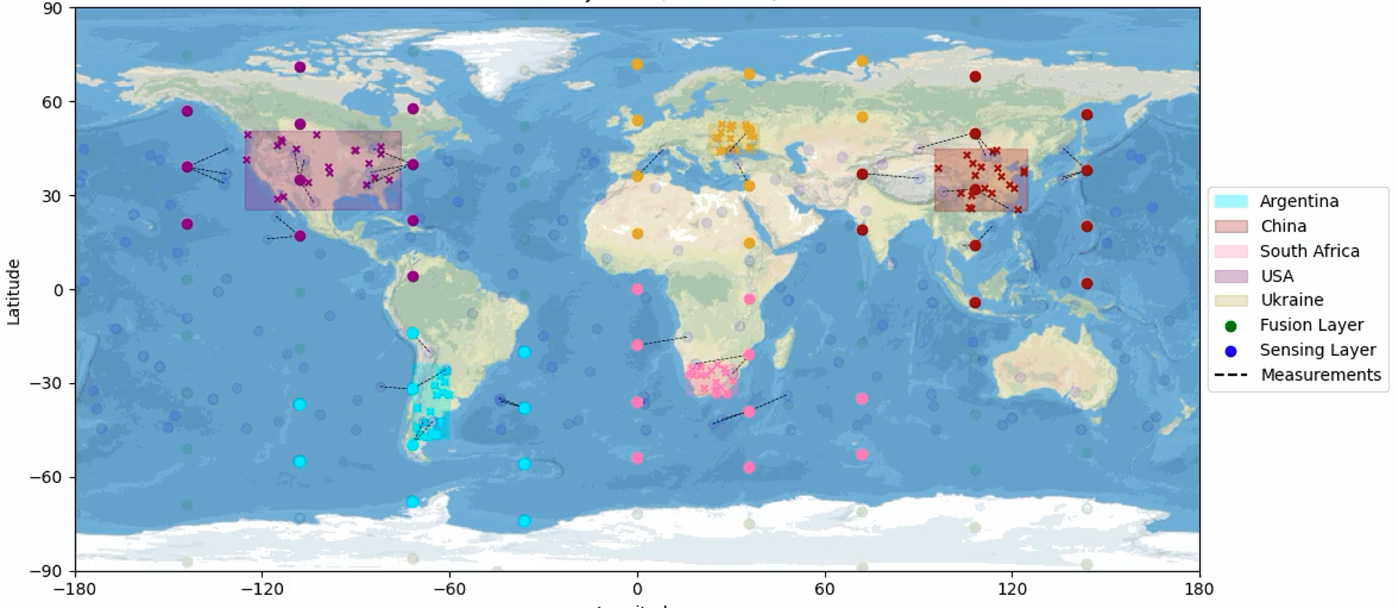
\includegraphics[width=0.8\textwidth]{figs/nominal_custody.png}
    \caption{Initial custody plan for an undercapacity case, 100 total targets, 20 in each country.}
    \label{fig:initial_custody_nominal}
\end{figure*}


\begin{figure*}[t]
    \centering
    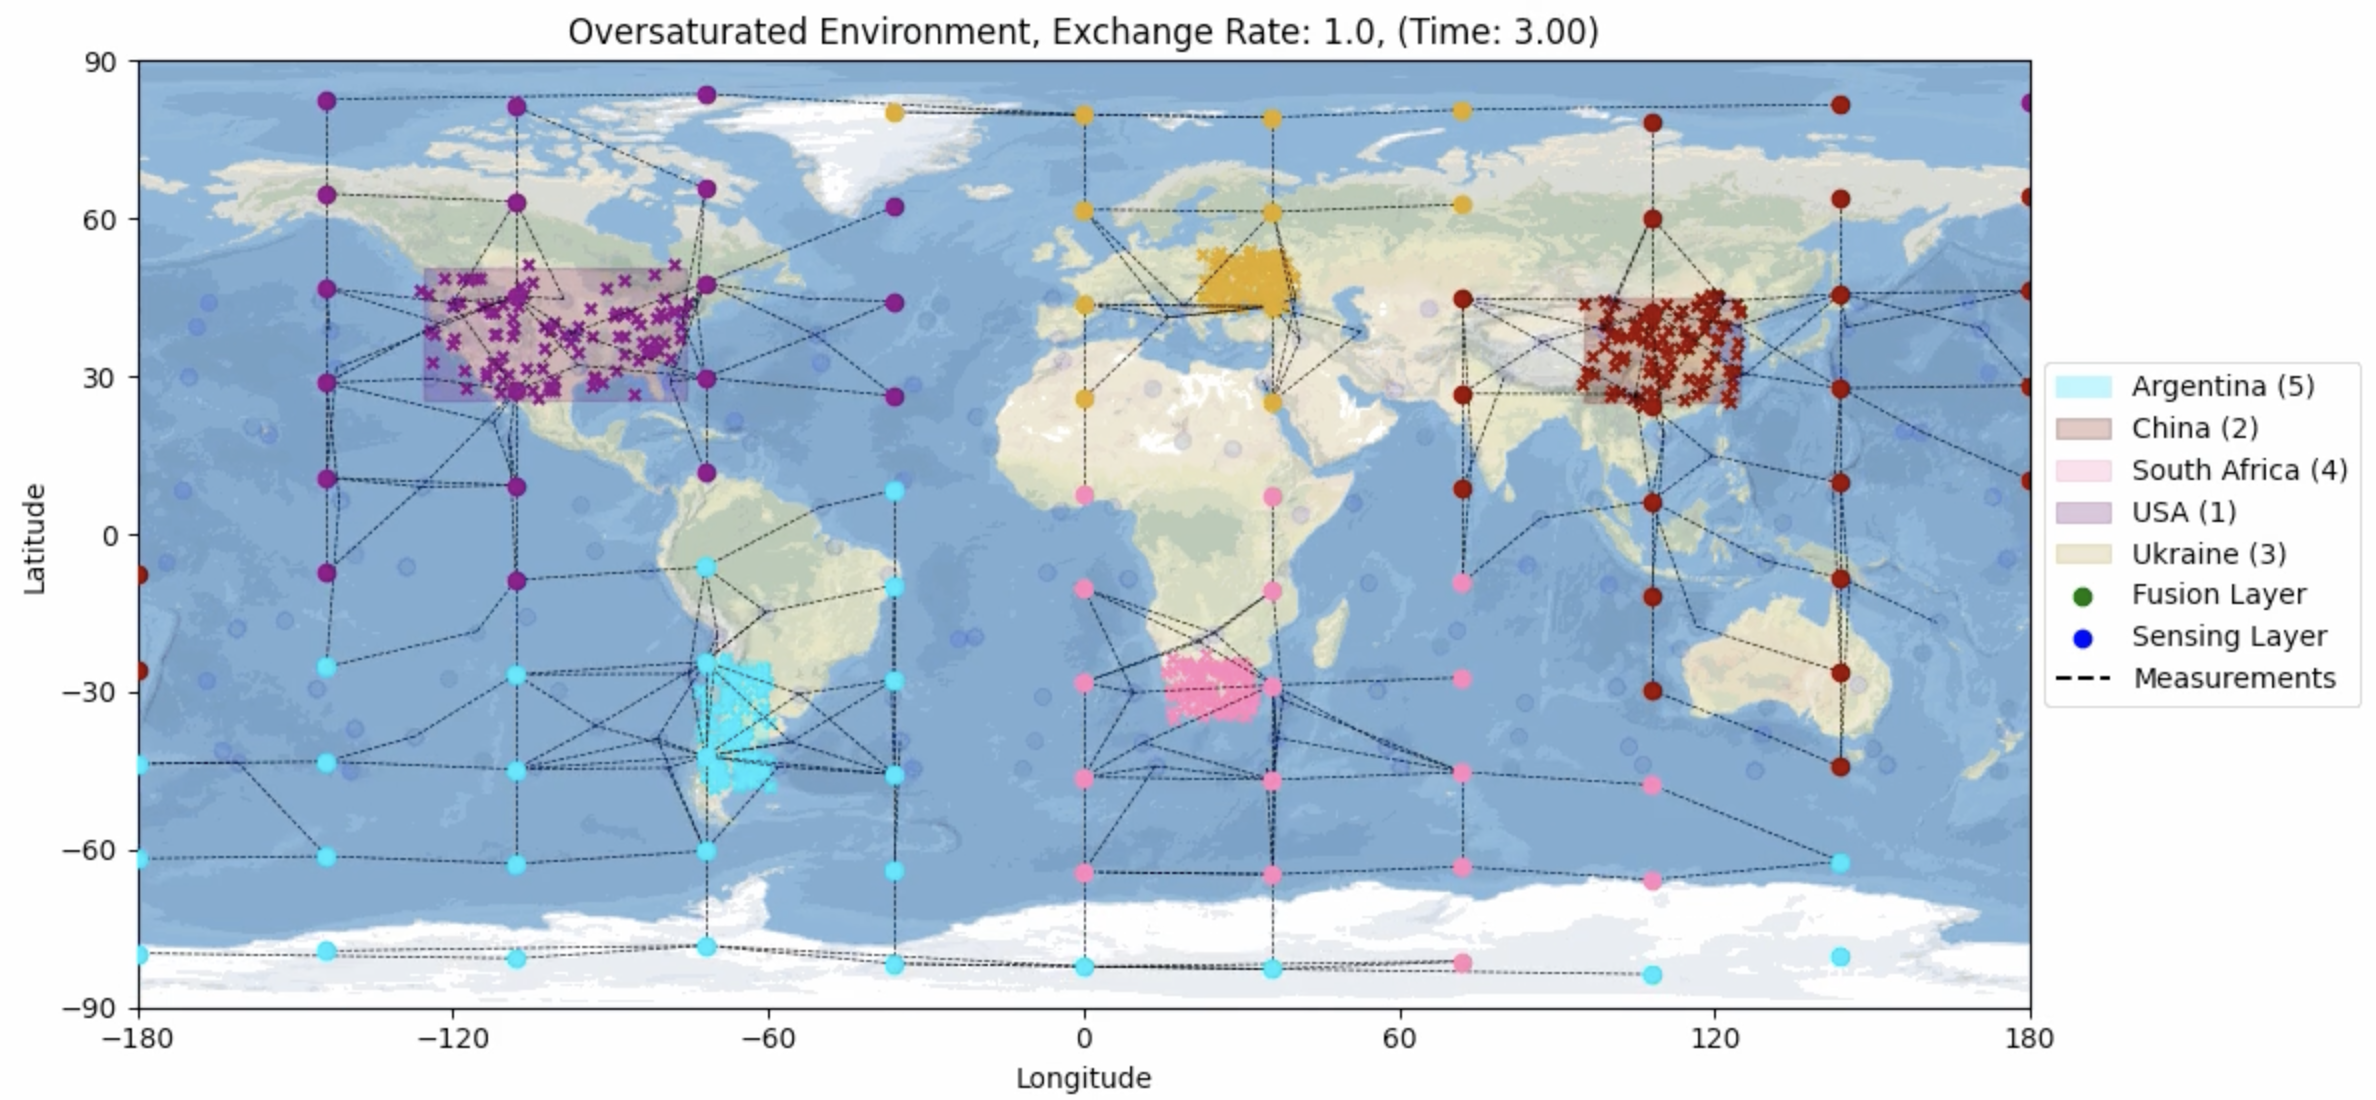
\includegraphics[width=0.8\textwidth]{figs/exchange_rate_1.png}
    \caption{Custody plan for overcapacity case, 500 targets, 200 target capacity, exchange rate of 1.}
    \label{fig:exchange_rate_1}
\end{figure*}

\begin{figure*}[t]
    \centering
    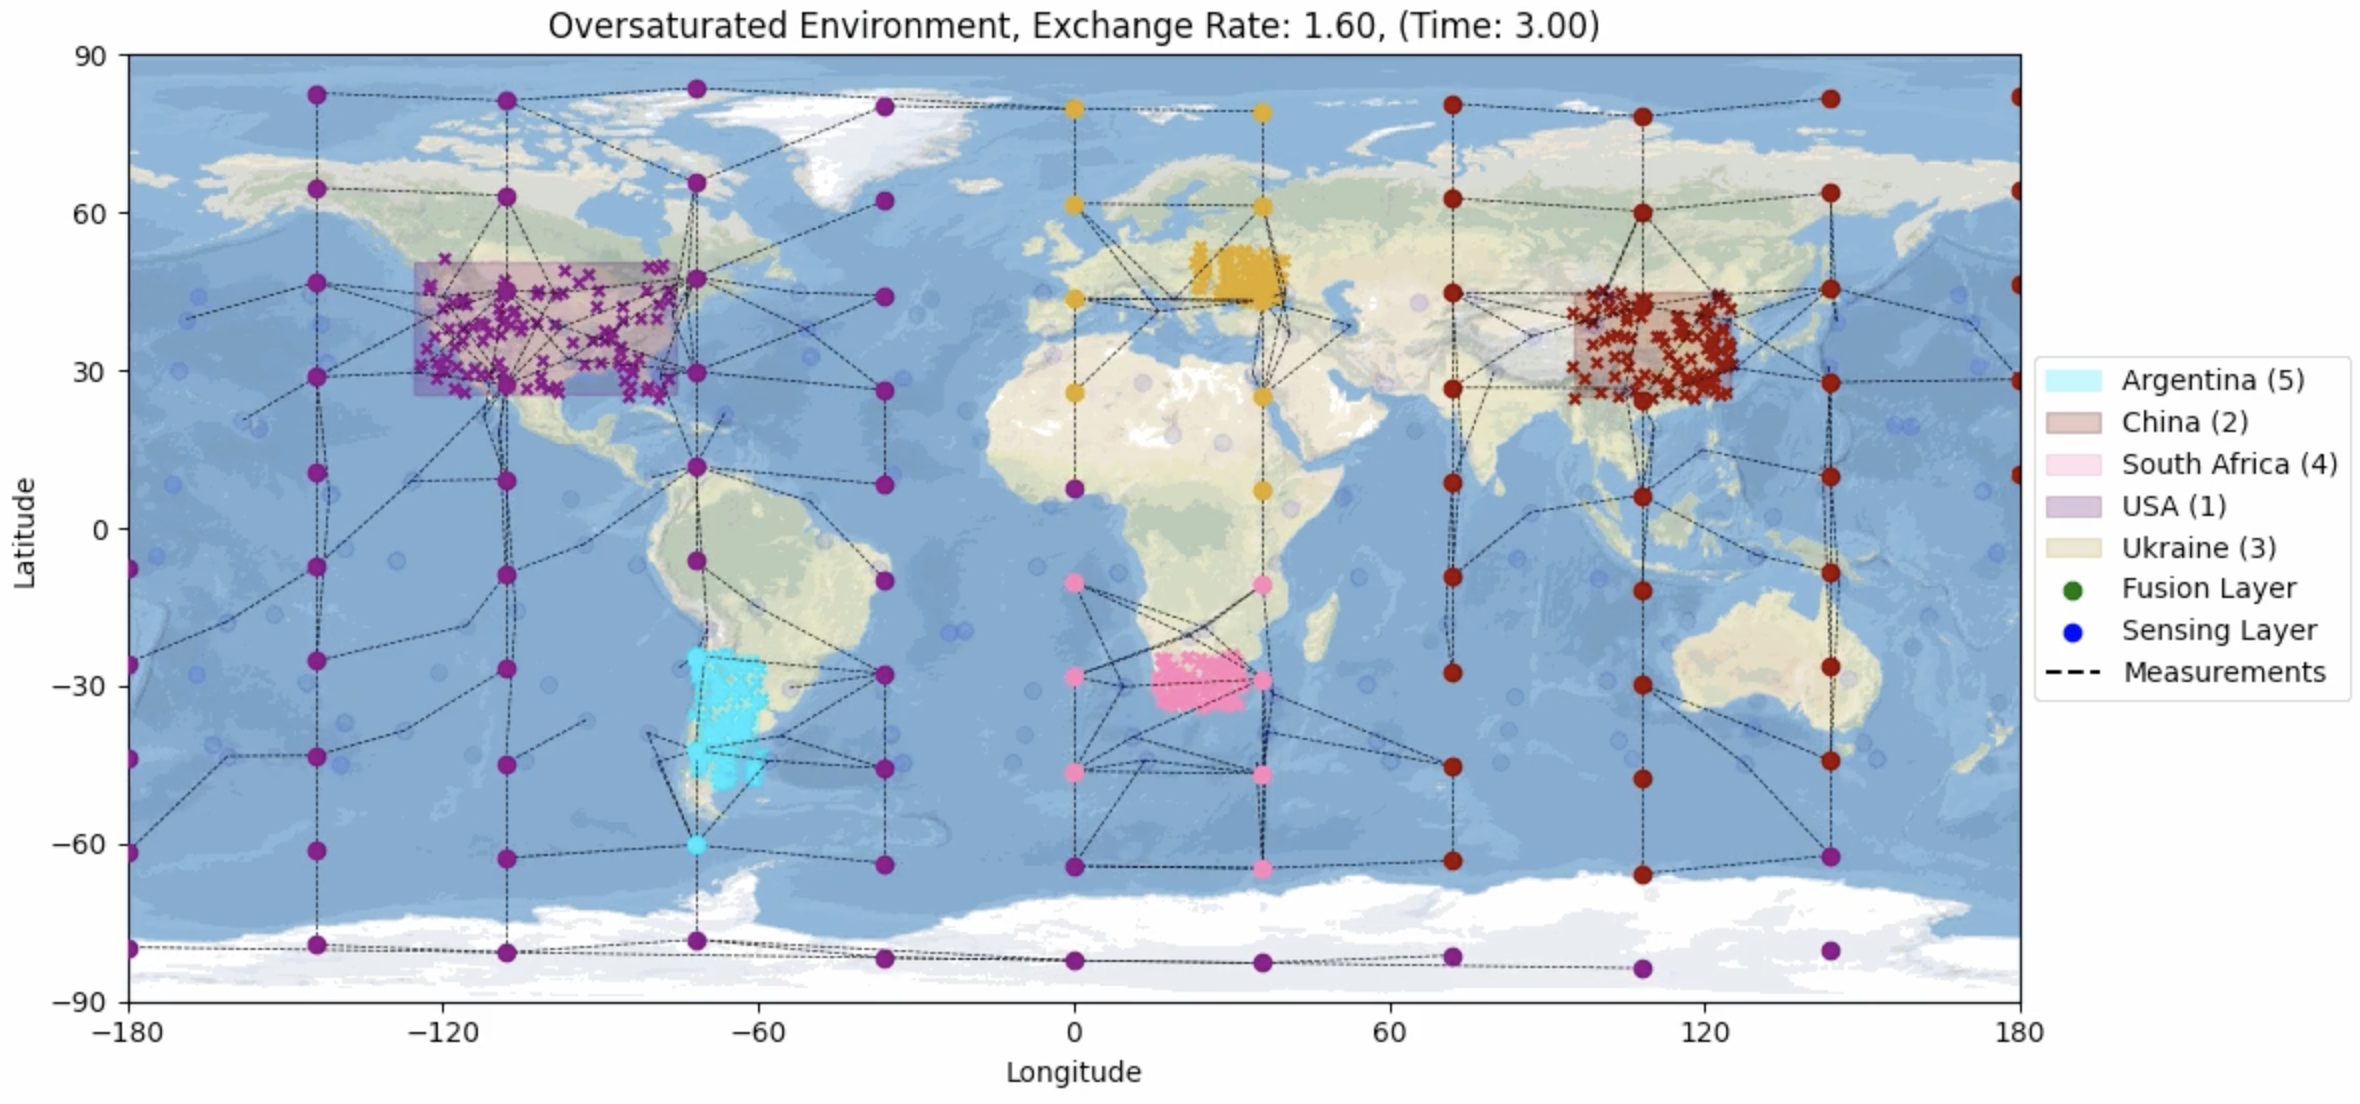
\includegraphics[width=0.8\textwidth]{figs/exchange_rate_1.6.png}
    \caption{Custody plan for overcapacity case, 500 targets, 200 target capacity, exchange rate of 1.6.}
    \label{fig:exchange_rate_1.6}
\end{figure*}
\begin{thebibliography}{00}

\bibitem{b1} M. E. Campbell and N. R. Ahmed, "Distributed Data Fusion: Neighbors, Rumors, and the Art of Collective Knowledge," IEEE Control Systems Magazine, vol. 36, no. 4, pp. 83-109, Aug. 2016.
\bibitem{b2} COIN-OR: Computational Infrastructure for Operations Research, "COIN-OR: Computational Infrastructure for Operations Research," 2024. [Online].
\bibitem{b3} "Decentralized Task Allocation Using Local Information Consistency Assumptions," Journal of Information Systems, 2024.
\bibitem{b4} R. Forsling, B. Noack, and G. Hendeby, "A Quarter Century of Covariance Intersection: Correlations Still Unknown? [Lecture Notes]," IEEE Control Systems Magazine, vol. 44, no. 2, pp. 81-105, Apr. 2024.
\bibitem{b5} S. J. Julier and J. K. Uhlmann, "A New Extension of the Kalman Filter to Nonlinear Systems," in Proc. SPIE 3068, Signal Processing, Sensor Fusion, and Target Recognition VI, 1997.
\bibitem{b6} S. Mitchell, M. O'Sullivan, and I. Dunning, "PuLP: A Linear Programming Toolkit for Python," The Python Papers, vol. 3, no. 1, 2011.
\bibitem{b7} H. Nabli, "An Overview on the Simplex Algorithm," Applied Mathematics and Computation, vol. 210, no. 2, pp. 479-489, Apr. 2009.
\bibitem{b8} R. T. Rockafellar and S. Uryasev, "Optimization of Conditional Value-at-Risk," The Journal of Risk, vol. 2, no. 3, pp. 21-41, 2000.
\bibitem{b9} W. J. Thompson, "Poisson Distributions," Computing in Science and Engineering, vol. 3, no. 3, pp. 78-82, May 2001.
\bibitem{b10} B. E. White, "Tactical Data Links, Air Traffic Management, and Software Programmable Radios," in 18th Digital Avionics Systems Conference Proceedings, St Louis, MO, 1999, pp. 5.C.5-1-5.C.5-8.

\end{thebibliography}

\end{document}
